\documentclass[conference]{IEEEtran}
\IEEEoverridecommandlockouts
% The preceding line is only needed to identify funding in the first footnote. If that is unneeded, please comment it out.
\usepackage{cite}
\usepackage{amsmath,amssymb,amsfonts}
\usepackage{algorithmic}
\usepackage{graphicx}
\graphicspath{{./images/}} % Specify the path to your images
\usepackage{textcomp}
\usepackage{xcolor}
\usepackage{url}
\def\BibTeX{{\rm B\kern-.05em{\sc i\kern-.025em b}\kern-.08em
    T\kern-.1667em\lower.7ex\hbox{E}\kern-.125emX}}
\begin{document}

\title{Forecasting a Caf\'e's Daily Ingredient Demand with Damped Triple Exponential Smoothing}

\author{\IEEEauthorblockN{Bastian Queckenstedt}
\IEEEauthorblockA{\textit{Department of Informatics} \\
\textit{Universit\"at Hamburg}\\
Hamburg, Germany \\
email address or ORCID}
\and
\IEEEauthorblockN{Tobias Christopher Kr\"oncke}
\IEEEauthorblockA{\textit{Department of Informatics} \\
\textit{Universit\"at Hamburg}\\
Hamburg, Germany \\
\url{https://orcid.org/0009-0004-4367-4395}}
\and
\IEEEauthorblockN{Efe Enes Nayci}
\IEEEauthorblockA{\textit{Department of Informatics} \\
\textit{Universit\"at Hamburg}\\
Hamburg, Germany \\
\url{https://orcid.org/0009-0000-9966-9115}}
}

\maketitle

\begin{abstract}
We present a lightweight forecasting pipeline that predicts the daily ingredient
demand of a caf\'e from its raw sales history. Per-drink sales records are loaded into
a relational database, joined with recipe data that is resolved into six base
ingredients, and aggregated into one daily time series per ingredient. A
self-implemented additive Holt--Winters model with a damped trend extrapolates each
series into the future. In a two-month validation window, the model achieves a mean
absolute percentage error of 14\% across all six ingredients, demonstrating that
classical exponential smoothing remains effective for small-scale retail demand
forecasting when transactional data must be translated through complex recipes.
\end{abstract}

\begin{IEEEkeywords}
forecasting, time series, triple exponential smoothing, Holt--Winters, damped trend, PostgreSQL
\end{IEEEkeywords}

\section{Introduction}
We present an end-to-end demonstration for a one-year sales log of a caf\'e
(3\,547 transactions, March 2024 to March 2025) provided as course
material\footnote{Datasets \emph{Coffee sales} and \emph{Coffee recipes} from the
course \emph{Databases and Information Systems}, Universit\"at Hamburg, summer term
2026.}. Sales and recipe data are integrated within a PostgreSQL database, aggregated
into daily ingredient-usage series, and forecast by an additive Holt--Winters model with
a damped trend, implemented from scratch. A command-line tool exposes every model
parameter to the user, enabling interactive exploration of the forecast behavior.

\section{Related Work}
Demand forecasting in food service has long relied on classical time-series methods
before the recent surge of deep-learning approaches. The Holt--Winters triple
exponential smoothing method~\cite{holt2004,winters1960} remains the standard baseline
for data with both trend and seasonality, and its damped variant~\cite{gardner1985}
addresses the common failure mode of linear trend extrapolation over long horizons.
Subsequent work~\cite{hyndman2008} formalized these methods within a state-space
framework and established error metrics such as MAE and RMSE as universal evaluation
criteria.

For small-scale operations without such auxiliary data, however,
single-database pipelines with classical smoothing remain cost-effective.
Our work shows that a self-contained PostgreSQL and Python stack with Holt--Winters
provides a practical baseline for caf\'e inventory management.

\section{Architecture Overview}
Figure~\ref{fig:architecture} illustrates the data pipeline. The raw sales file
\texttt{Coffee\_sales.csv} is copied verbatim into the relational table
\texttt{coffee\_sales} in PostgreSQL; the CSV file is never accessed again, and all
subsequent queries operate on the database alone.

\begin{figure}[htbp]
\centerline{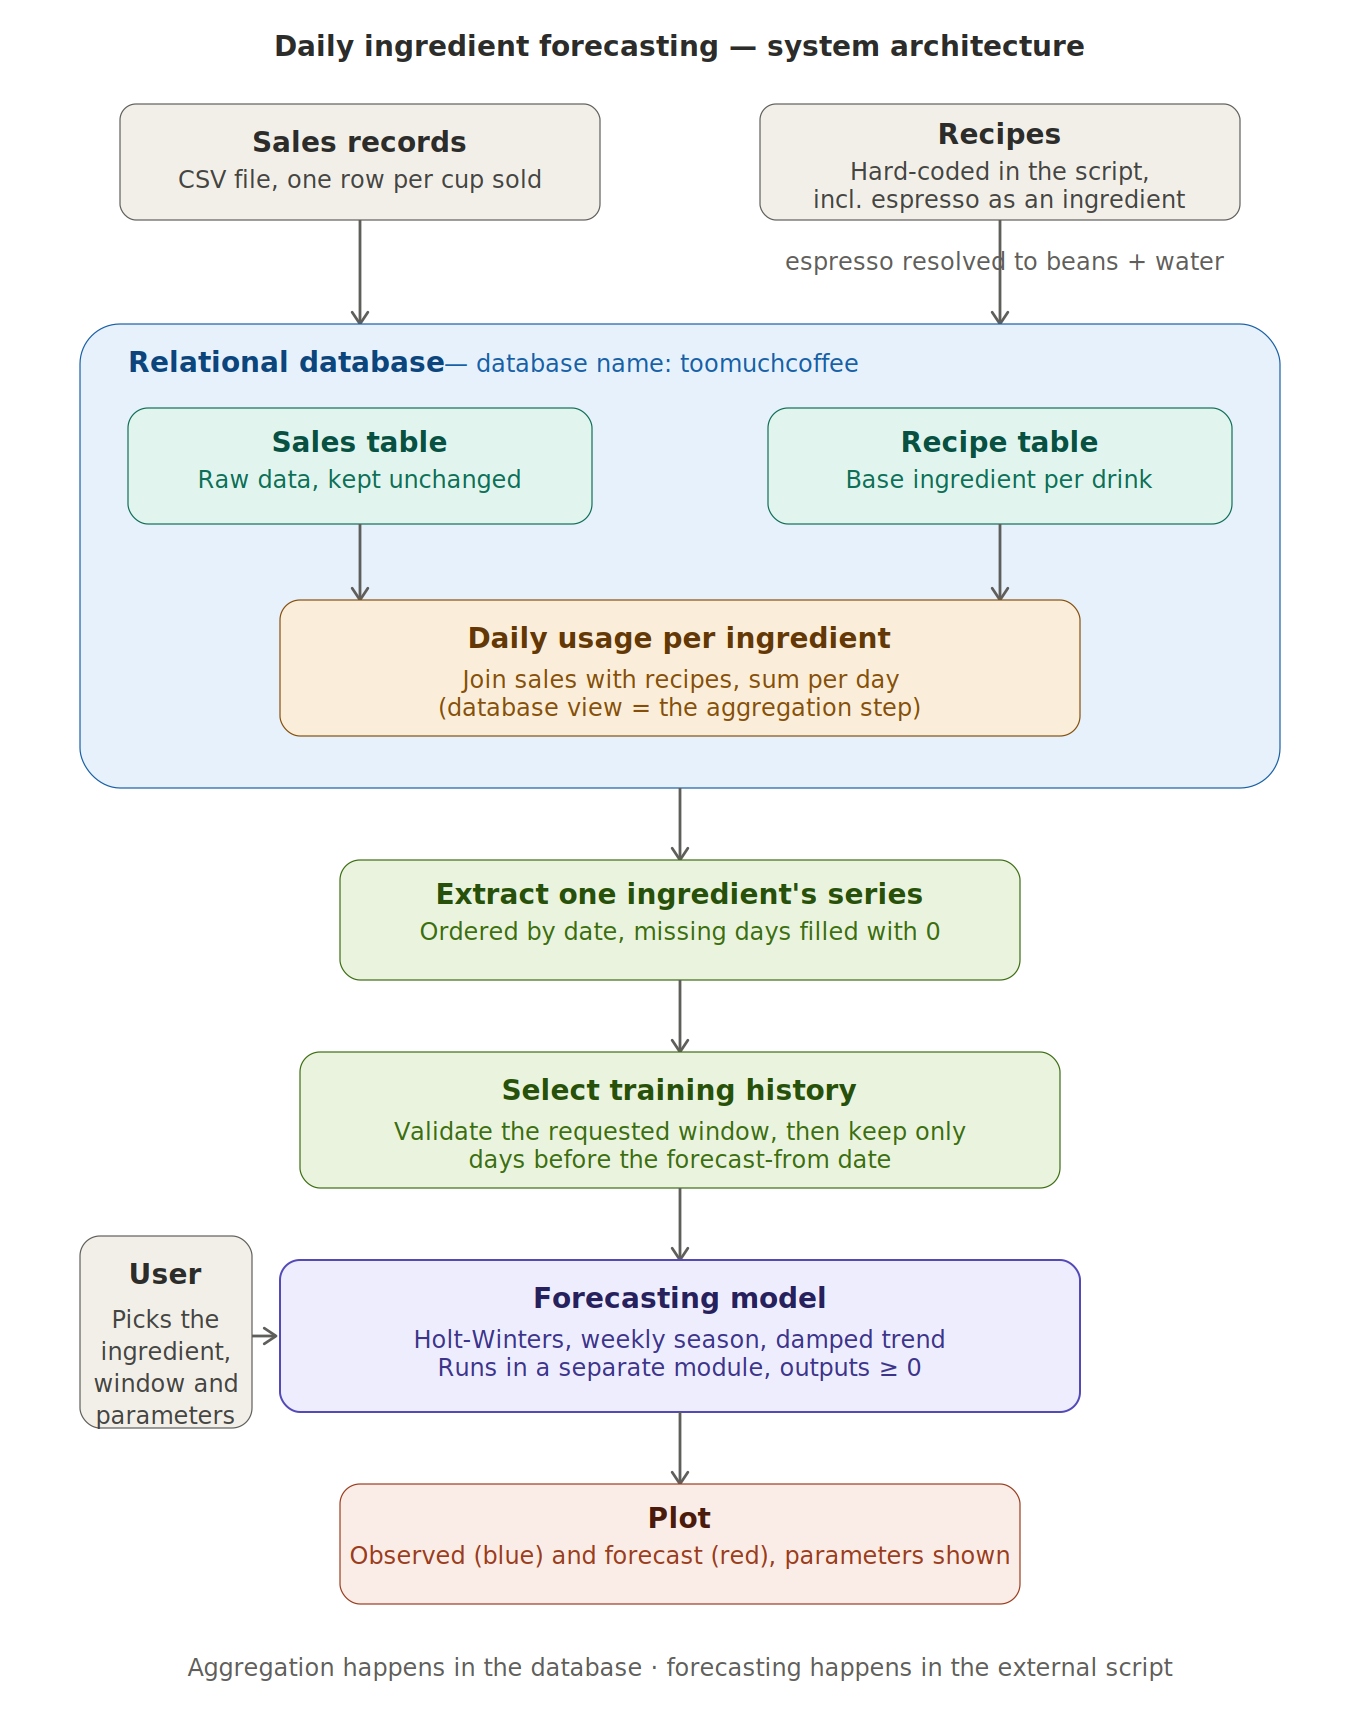
\includegraphics[width=0.74\columnwidth]{dis_architecture.png}}
\caption{Architecture of the demonstration: sales and recipe data are integrated in
PostgreSQL, aggregated by a view, and consumed by the Python forecasting tool.}
\label{fig:architecture}
\end{figure}

The recipes are derived from the completed JSON document collection of the second
exercise sheet and embedded as a constant within the loader script. During loading, the
pseudo-ingredient \emph{espresso shot} is recursively resolved into its base ingredients
(18\,g coffee beans and 30\,ml water per shot). A SQL view
\texttt{daily\_ingredient\_usage} joins the recipe table with the sales table and aggregates
per day and ingredient. The Python forecasting tool extracts one ingredient's
time series from this view, fills days without sales with zero, forecasts the series, and
renders the plot using \texttt{matplotlib}.

\subsection{Forecasting Approach}
We employ additive triple exponential smoothing (the Holt--Winters
method)~\cite{holt2004,winters1960,hyndman2021fpp3} with a seasonality period of $m=7$ days, reflecting
the pronounced weekly pattern in the data, extended by a damped trend~\cite{gardner1985,hyndman2021fpp3}.
Given smoothing factors $\alpha,\beta,\gamma \in [0,1]$ and a damping factor
$\phi \in (0,1]$, the level $\ell_t$, trend $b_t$, and seasonal component $s_t$ are
updated for each observation $x_t$ as follows:
\begin{align}
\ell_t &= \alpha (x_t - s_{t-m}) + (1-\alpha)(\ell_{t-1} + \phi b_{t-1}),\\
b_t &= \beta (\ell_t - \ell_{t-1}) + (1-\beta)\,\phi b_{t-1},\\
s_t &= \gamma (x_t - \ell_t) + (1-\gamma)\,s_{t-m},
\end{align}
and the $h$-step-ahead forecast is given by
$\hat{x}_{T+h} = \ell_T + (\sum_{i=1}^{h}\phi^{i})\,b_T + s_{T-m+1+((h-1) \bmod m)}$.
Damping ($\phi<1$) causes the trend to asymptotically approach a plateau rather than
extrapolating linearly, which preserves the plausibility of long-horizon forecasts;
setting $\phi=1$ recovers the classical undamped model. The recursion is implemented in
pure Python without reliance on any external forecasting library.

\section{Demonstration Proposal}
The demonstration comprises an interactive command line session accompanied by live
plots. Users first observe a preconfigured forecast and subsequently modify parameters
to immediately observe the model's response.

\subsection{Setup}\label{subsec:setup}
The demonstration executes locally with PostgreSQL and Python
3.12, utilizing \texttt{psycopg2}, \texttt{argparse}, and
\texttt{matplotlib}. A complete execution finishes in well under one second.

\subsection{User Experience}
Users interact with the tool through command line flags: \texttt{-i} selects among the
six ingredients, \texttt{--forecast\_from} and \texttt{--forecast\_until} define the
inclusive forecast window, and \texttt{-a}, \texttt{-b}, \texttt{-g}, \texttt{-p}
control $\alpha$, $\beta$, $\gamma$, and $\phi$, respectively.

Two scenarios structure the walkthrough. The first, \emph{validation}, positions the
forecast window within the observed data range, such that the model sees only the history
preceding the window; the resulting prediction can then be compared visually against
actual values (Fig.~\ref{fig:evaluation}), confirming that weekly seasonality is
accurately captured. Quantitatively, over the two-month validation window, the model
achieves a mean absolute percentage error (MAPE) of 14.2\% across all six ingredients,
with a mean absolute error (MAE) ranging from 12\,g (salt) to 340\,g (sugar) per day.
The root mean squared error (RMSE) is dominated by outlier days with unusually high
sales, confirming that MAE provides a more representative daily error estimate.
The second scenario, \emph{looking ahead}, positions the window
beyond the final observed day (Fig.~\ref{fig:future}). Users are then invited to explore
interactively -- for instance, by switching to milk, setting $\phi=1$ to observe the
undamped trend drift across a long horizon, or setting $\alpha=1$ to observe the
forecast tracking noise rather than signal.

\begin{figure}[htbp]
\centerline{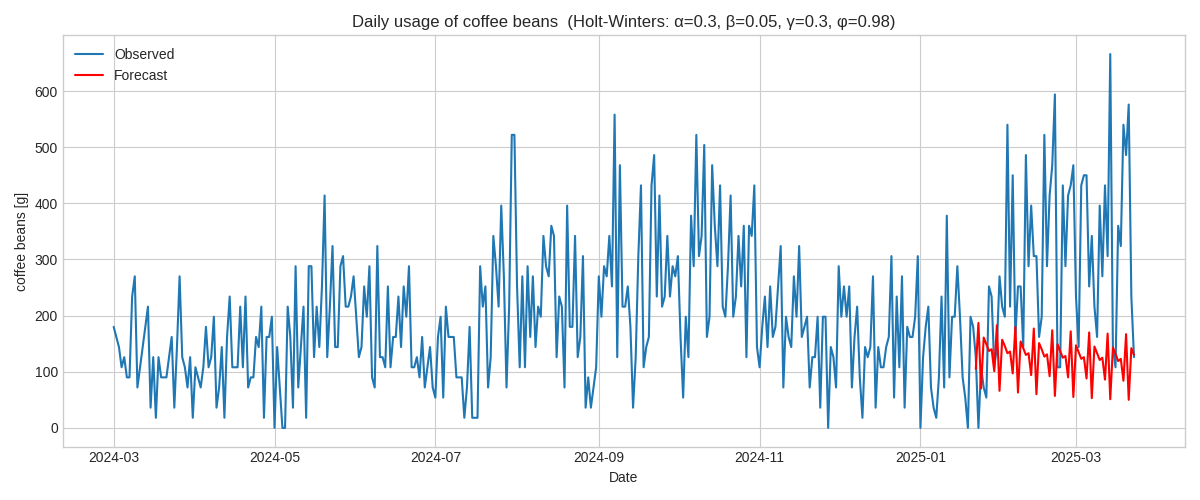
\includegraphics[width=\columnwidth]{forecast_evaluation_coffee_beans_2025-01-22_2025-03-23_a03_b005_g03_p098.png}}
\caption{Validation: forecast (red) of the last two observed months of coffee-bean
usage, computed exclusively from the history preceding the window
($\alpha{=}0.3$, $\beta{=}0.05$, $\gamma{=}0.3$, $\phi{=}0.98$).}
\label{fig:evaluation}
\end{figure}

\begin{figure}[htbp]
\centerline{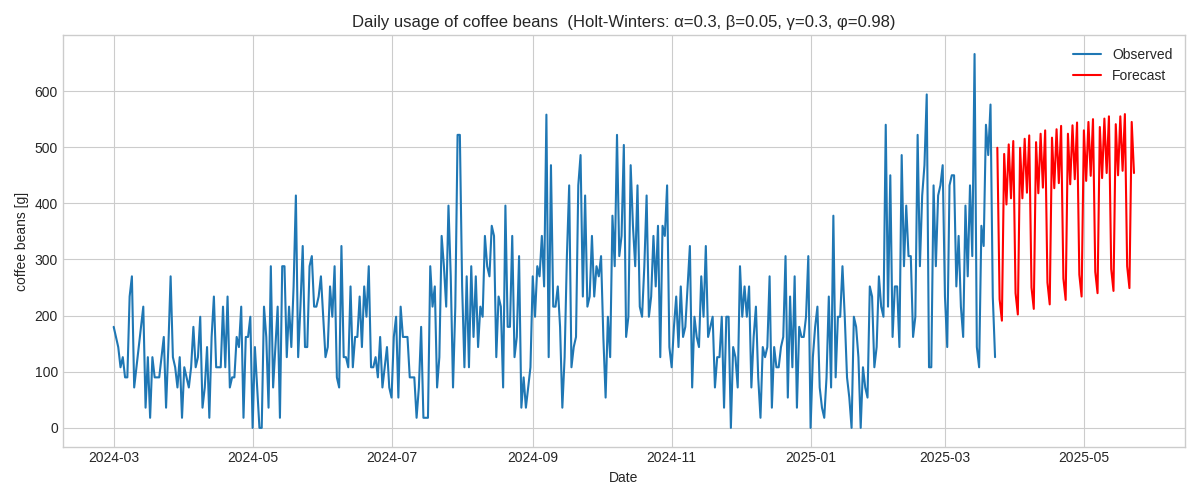
\includegraphics[width=\columnwidth]{forecast_future_coffee_beans_2025-03-24_2025-05-23_a03_b005_g03_p098.png}}
\caption{Looking ahead: two-month forecast extending beyond the observed data, using the
same parameters as in Fig.~\ref{fig:evaluation}.}
\label{fig:future}
\end{figure}

\subsection{Conclusion}
The demonstration illustrates that a complete ingredient-demand forecasting pipeline
requires minimal infrastructure: a single relational database, one SQL view for
drink-to-ingredient translation, and approximately one hundred lines of custom-implemented
Holt--Winters code. Its distinguishing characteristic is full parameter transparency --
every smoothing factor is exposed as a command-line argument, transforming the
demonstration into an interactive platform for exploring exponential smoothing.

\section*{Limitations and Discussion}
The demonstration shows that Holt--Winters smoothing provides a reasonable baseline
for caf\'e ingredient forecasting, but several limitations apply. First, the model
cannot account for one-off events such as holidays or special promotions~\cite{box2015}.
Second, the deterministic recipe resolution does not capture substitution behavior,
introducing systematic bias. Third, with only 3\,547 transactions over one year, the
data is too small for more complex models such as SARIMAX. Finally, the damping
parameter $\phi$ was held fixed at 0.98; per-ingredient optimization could further
reduce the MAPE.

\section*{Acknowledgment}
Portions of the source code were developed with the assistance of Anthropic's large
language model, Claude, and subsequently reviewed by the authors.

\begin{thebibliography}{9}
\bibitem{hyndman2021fpp3} R.~J. Hyndman and G.~Athanasopoulos,
\emph{Forecasting: Principles and Practice}, 3rd~ed. Melbourne, Australia: OTexts, 2021,
ch.~8.3. [Online]. Available: \url{https://otexts.com/fpp3/holt-winters.html}
\bibitem{holt2004} C.~C. Holt, ``Forecasting seasonals and trends by exponentially
weighted moving averages,'' \emph{International Journal of Forecasting}, vol.~20,
no.~1, pp. 5--10, 2004, reprint of ONR Research Memorandum 52, Carnegie Institute
of Technology, 1957.
\bibitem{winters1960} P.~R. Winters, ``Forecasting sales by exponentially weighted
moving averages,'' \emph{Management Science}, vol.~6, no.~3, pp. 324--342, 1960.
\bibitem{gardner1985} E.~S. Gardner, Jr. and E.~McKenzie, ``Forecasting trends in
time series,'' \emph{Management Science}, vol.~31, no.~10, pp. 1237--1246, 1985.
\bibitem{hyndman2008}
R.~J. Hyndman, A.~B. Koehler, J.~K. Ord, and R.~D. Snyder,
\emph{Forecasting with Exponential Smoothing: The State Space Approach}.
Berlin, Germany: Springer, 2008.
\bibitem{box2015} G.~E.~P. Box, G.~M. Jenkins, G.~C. Reinsel, and G.~M. Ljung,
\emph{Time Series Analysis: Forecasting and Control}, 5th~ed. Hoboken, NJ, USA: Wiley, 2015.
\end{thebibliography}

\end{document}
